\documentclass[11pt,a4paper]{article}

% ---------------------------------------------------------------------------
%  Thermal Physics revision guide -- Alex lessons 9--10 July 2026
%  Prepared for Phuc Nguyen. Edexcel IAL Physics (Unit 5 Thermodynamics).
%  Clean serious black-and-white academic style. Compile with XeLaTeX x2.
% ---------------------------------------------------------------------------

\usepackage{fontspec}
\usepackage{amsmath,amssymb}
\usepackage{siunitx}
\usepackage{booktabs}
\usepackage{array}
\usepackage{enumitem}
\usepackage{graphicx}
\usepackage{tikz}
\usepackage{pgfplots}
\pgfplotsset{compat=1.17}
\usetikzlibrary{arrows.meta,positioning,decorations.pathmorphing,calc,patterns,shapes.geometric}
\usepackage[most]{tcolorbox}
\usepackage{fancyhdr}
\usepackage{longtable}
\usepackage[a4paper,margin=2.2cm,headheight=14pt]{geometry}
\usepackage[hidelinks]{hyperref}
\usepackage{microtype}
\usepackage{titlesec}

% ---------------------------------------------------------------------------
%  Colours: strictly black / grey
% ---------------------------------------------------------------------------
\definecolor{guidegrey}{gray}{0.45}
\definecolor{lightgrey}{gray}{0.93}
\definecolor{midgrey}{gray}{0.75}
\definecolor{boxback}{gray}{0.97}

% ---------------------------------------------------------------------------
%  siunitx set-up
% ---------------------------------------------------------------------------
\sisetup{per-mode=symbol, inter-unit-product=\ensuremath{\,}}
\DeclareSIUnit\celsius{\degreeCelsius}

% ---------------------------------------------------------------------------
%  Headers / footers
% ---------------------------------------------------------------------------
\pagestyle{fancy}
\fancyhf{}
\renewcommand{\headrulewidth}{0.4pt}
\renewcommand{\footrulewidth}{0.0pt}
\fancyhead[L]{\small\itshape Thermal Physics --- Edexcel IAL}
\fancyhead[R]{\small\itshape Alex lessons, 9--10 July 2026}
\fancyfoot[C]{\small\thepage}

% ---------------------------------------------------------------------------
%  Section formatting
% ---------------------------------------------------------------------------
\titleformat{\section}{\Large\bfseries}{\thesection}{0.7em}{}[{\titlerule[0.8pt]}]
\titleformat{\subsection}{\large\bfseries}{\thesubsection}{0.6em}{}
\titleformat{\subsubsection}{\normalsize\bfseries}{\thesubsubsection}{0.5em}{}

% ---------------------------------------------------------------------------
%  Custom boxes (thin black / grey only)
% ---------------------------------------------------------------------------
\newtcolorbox{keybox}[1][]{
  enhanced, colback=boxback, colframe=black, boxrule=0.6pt,
  arc=1pt, left=6pt,right=6pt,top=5pt,bottom=5pt,
  fonttitle=\bfseries, coltitle=black, title={#1},
  breakable}

\newtcolorbox{plainbox}{
  enhanced, colback=white, colframe=guidegrey, boxrule=0.5pt,
  arc=1pt, left=6pt,right=6pt,top=5pt,bottom=5pt, breakable}

\newtcolorbox{defbox}[1][Definition]{
  enhanced, colback=lightgrey, colframe=black, boxrule=0.7pt,
  arc=0pt, left=6pt,right=6pt,top=5pt,bottom=5pt,
  fonttitle=\bfseries, title={#1}, breakable}

\newtcolorbox{watchbox}{
  enhanced, colback=white, colframe=black, boxrule=0.5pt,
  sharp corners, left=6pt,right=6pt,top=5pt,bottom=5pt, breakable}

\newtcolorbox{advicebox}{
  enhanced, colback=boxback, colframe=guidegrey, boxrule=0.5pt,
  arc=1pt, left=6pt,right=6pt,top=4pt,bottom=4pt, breakable}

% shorthand
\newcommand{\ts}[1]{\textup{[#1]}}       % timestamp tag
\newcommand{\dtheta}{\Delta\theta}
\newcommand{\dE}{\Delta E}

% explicit image path helpers (both folders contain identically-named files)
\newcommand{\imgA}[1]{images/2026-07-09/#1}
\newcommand{\imgB}[1]{images/2026-07-10/#1}

% ---------------------------------------------------------------------------
\begin{document}

% =====================  TITLE PAGE  =====================
\begin{titlepage}
\centering
\vspace*{1.2cm}
{\Large\scshape Edexcel International A Level Physics}\\[0.4cm]
{\large Unit 5 --- Thermodynamics (Thermal Energy Transfer)}\\[1.6cm]
\rule{\textwidth}{1.1pt}\\[0.5cm]
{\huge\bfseries Thermal Physics}\\[0.35cm]
{\Large Infrared, Conduction, Convection, Insulation,\\[0.15cm]
Specific Heat Capacity, Latent Heat and Gas Pressure}\\[0.5cm]
\rule{\textwidth}{1.1pt}\\[1.6cm]

{\large A complete lecture-replacement revision guide}\\[0.3cm]
{\large reconstructed from two consecutive lessons with Alex}\\[1.2cm]

\begin{tabular}{rl}
\textbf{Lessons:} & 9 July 2026 (\SI{60}{min}) and 10 July 2026 (\SI{49}{min})\\[4pt]
\textbf{Prepared for:} & Phuc Nguyen\\[4pt]
\textbf{Board:} & Pearson Edexcel IAL Physics (with ESAT/GCSE foundations)\\[4pt]
\textbf{Chapter scope:} & One coherent thermal-physics chapter\\
 & (10 July continues 9 July)\\
\end{tabular}

\vfill
{\small This guide reconstructs both lessons from timestamped lesson transcripts,
watched-video analyses of the recordings, and the exact board screenshots shared during
the sessions, corrected against the Edexcel textbook, SaveMyExams packs and the official
IAL specification. See the source register in Section~\ref{sec:sources}.}
\vspace{1cm}
\end{titlepage}

% =====================  CONTENTS  =====================
\tableofcontents
\thispagestyle{fancy}
\clearpage

% ===========================================================================
\section{Specification and honest source register}
\label{sec:sources}
% ===========================================================================

\subsection{Where these lessons sit on the Edexcel IAL specification}

Both lessons belong to \textbf{Unit 5: Thermodynamics, Radiation, Oscillations and
Cosmology} (an IA2 compulsory, externally assessed unit; \SI{1}{hour}\,\SI{45}{min},
90 marks). The thermal-transfer material Alex taught is the qualitative and
calculation-based foundation on which the Unit~5 thermal spec points build. The lessons
also deliberately revisit GCSE/ESAT ideas (energy stores, heat-transfer descriptions,
insulation) because the examiner rewards \emph{accurate process descriptions}, and
because the ESAT admissions test draws on the same physics.

\begin{keybox}[Spec points 125--132 --- the thermodynamics core these lessons feed into]
The Edexcel IAL thermodynamics strand (spec points numbered 125--132 in the
unit sequence) covers:
\begin{itemize}[leftmargin=1.4em,itemsep=1pt]
  \item \textbf{125} --- internal energy as the sum of the random kinetic and potential
        energies of a body's particles.
  \item \textbf{126} --- absolute zero (\SI{0}{K}) and the Kelvin scale; a change of
        \SI{1}{K} equals a change of \SI{1}{\celsius}.
  \item \textbf{127} --- specific heat capacity: $\dE = mc\,\dtheta$.
  \item \textbf{128} --- specific latent heat of fusion and vaporisation:
        $\dE = L\,\Delta m$; no temperature change during a change of state.
  \item \textbf{129--130} --- the gas laws (Boyle, pressure, Charles) and the ideal-gas
        equation $pV = NkT$.
  \item \textbf{131} --- the kinetic-theory model of gas pressure and
        $\tfrac{1}{2}m\langle c^2\rangle = \tfrac{3}{2}kT$.
  \item \textbf{132} --- root-mean-square speed and the link between mean molecular
        kinetic energy and absolute temperature.
\end{itemize}
The \emph{qualitative} thermal-transfer content (infrared, conduction, convection,
insulation) is examined mainly through worded explanation questions and through the
"controlling heat transfer" practical context that Alex used. It is spec-adjacent
GCSE/ESAT foundation that Unit~5 assumes you already command.
\end{keybox}

\subsection{Honest source register and confidence notes}

This guide was built from the following evidence, in the priority order Alex's board
work demands. Everything below is stated plainly so you know exactly what is
high-confidence lesson fact and what is reconstruction.

\begin{longtable}{@{}p{3.4cm}p{2.0cm}p{9.3cm}@{}}
\toprule
\textbf{Source} & \textbf{Status} & \textbf{What it gives / confidence} \\
\midrule
\endhead
Lesson transcripts (both days) & \textbf{Pass} & Complete timestamped transcripts:
9 July (274 segments, ending \ts{01:00:25}); 10 July (213 segments, ending
\ts{48:40}). \emph{Highest} trust for spoken wording and instructions. Speaker labels
were inferred from dialogue; a few words are ASR-uncertain and are flagged as such. \\
\addlinespace
Board screenshots & \textbf{Pass} & All 19 images (9 July: 12; 10 July: 7) downloaded
and read. \emph{Highest} trust for exact question text, numbers, units and diagrams.
Pen-colour authorship is \emph{not} used to assign mistakes. \\
\addlinespace
Video analysis & \textbf{Pass} & Both recordings analysed for chronology and
audio/visual context. Used for ordering and gesture, \emph{not} for exact numbers where
a screenshot or transcript exists. \\
\addlinespace
Edexcel textbook (Yr 2, ch.\ 10--12) & \textbf{Pass} & Used to correct physics and set
IAL scope (SHC, latent heat, gas laws, kinetic theory). \\
\addlinespace
SaveMyExams packs & \textbf{Pass} & Thermal Energy Transfer + Kinetic Theory/Ideal
Gases, including core-practical detail and examiner tips. \\
\addlinespace
Official IAL spec excerpt & \textbf{Pass} & Unit~5 description and formula context. \\
\addlinespace
OneNote (Alex's notebook) & \textbf{Attempted --- no matching page} & Alex's mounted
\textit{Phuc-Physics} OneNote contains Mechanics, Materials, Work/Energy/Power, Waves
and Electricity, \textbf{but no thermal teaching page}. Only its admin
\textit{Spec} and \textit{Formula Sheet} pages were available and used. There was no
thermal OneNote lesson page, and this guide does not pretend otherwise. \\
\addlinespace
Prior thermal guide & \textbf{Checked --- absent} & No earlier 9--10 July thermal guide
exists; none is claimed as a source. \\
\bottomrule
\end{longtable}

\begin{plainbox}
\textbf{Date-label note.} The 10 July lesson's message caption reads "june 10th," but the
message timestamp and the lesson-recording title both confirm the true date is
\textbf{10 July 2026}. This guide follows the true date throughout.

\smallskip
\textbf{Attribution rule.} Throughout, a mistake is labelled a "Phuc mistake" only where
the transcript or video directly evidences Phuc saying it. Where a board mark is
merely crossed out with no spoken owner, it is reported as a board correction event, not
assigned to anyone.
\end{plainbox}

\clearpage
% ===========================================================================
\section{One-page executive summary}
% ===========================================================================

\begin{keybox}[If you remember nothing else]
\begin{enumerate}[leftmargin=1.4em,itemsep=2pt]
  \item \textbf{Thermal energy} is a \emph{store} you can measure; \textbf{heating} is the
        \emph{transfer} of that energy from hot to cold. Never say "heat" for both.
  \item Energy always flows \textbf{hot $\to$ cold} until \textbf{thermal equilibrium}
        (equal temperatures).
  \item \textbf{Three transfer mechanisms:} conduction (particle vibrations / free
        electrons, mainly solids), convection (bulk flow of a heated fluid), radiation
        (infrared, needs no medium --- works across a vacuum).
  \item \textbf{All objects emit and absorb infrared all the time}; hotter objects emit
        more. Only at \textbf{\SI{0}{K}} would emission stop.
  \item \textbf{Black/matt} = best emitter \emph{and} best absorber. \textbf{White/shiny}
        = worst emitter/absorber, best reflector. Emission $\ne$ reflection.
  \item \textbf{Insulation} traps air: fewer particles $\Rightarrow$ less conduction;
        immobilised pockets $\Rightarrow$ no convection. Vacuum is the ideal (no
        particles), silver/foil reflects infrared.
  \item In a \textbf{vacuum} (space) there is no conduction and no convection, so a
        machine can only lose heat by \textbf{radiation} --- space does not automatically
        cool it.
\end{enumerate}
\end{keybox}

\begin{keybox}[Formulae to command]
\begin{center}
\renewcommand{\arraystretch}{1.5}
\begin{tabular}{@{}p{4.7cm}p{5.3cm}p{4.6cm}@{}}
\toprule
\textbf{Quantity} & \textbf{Equation} & \textbf{Units} \\
\midrule
Pressure & $p = \dfrac{F}{A}$ & \si{\pascal} $=$ \si{\newton\per\metre\squared} \\
Specific heat capacity & $\dE = mc\,\dtheta$ & $c$ in \si{\joule\per\kilogram\per\kelvin} \\
Specific latent heat & $\dE = L\,\Delta m$ & $L$ in \si{\joule\per\kilogram} \\
Ideal gas & $pV = NkT$ & $k = \SI{1.38e-23}{\joule\per\kelvin}$ \\
Pressure law (fixed $V$) & $\dfrac{p_1}{T_1} = \dfrac{p_2}{T_2}$ & $T$ in \si{\kelvin} \\
Mean molecular KE & $\tfrac{1}{2}m\langle c^2\rangle = \tfrac{3}{2}kT$ & $T$ in \si{\kelvin} \\
\bottomrule
\end{tabular}
\end{center}
\end{keybox}

\begin{keybox}[Process triggers --- which mechanism is being tested?]
\begin{itemize}[leftmargin=1.4em,itemsep=1pt]
  \item "Passing vibrations / collisions of particles / through a solid" $\Rightarrow$
        \textbf{conduction}.
  \item "Electromagnetic waves / infrared / across empty space / surface colour"
        $\Rightarrow$ \textbf{radiation}.
  \item "A fluid (liquid or gas) rises/sinks / whole volumes of air move / a draught"
        $\Rightarrow$ \textbf{convection}.
  \item "\,$1$ kg\,\ldots\ by $1$ K, no state change" $\Rightarrow$ \textbf{specific
        heat capacity}. "\,change of state, constant temperature" $\Rightarrow$
        \textbf{latent heat}.
\end{itemize}
\end{keybox}

\begin{keybox}[Core definitions to memorise word-perfectly]
\textbf{Specific heat capacity:} the energy needed to raise the temperature of
\SI{1}{\kilogram} of a substance by \SI{1}{\kelvin} (or \SI{1}{\celsius}).

\textbf{Specific latent heat:} the energy needed to change the state of \SI{1}{\kilogram}
of a substance \emph{with no change in temperature} (fusion = solid$\leftrightarrow$liquid;
vaporisation = liquid$\leftrightarrow$gas).

\textbf{Thermal equilibrium:} the state reached when a body radiates energy at the same
rate as it absorbs it, so its temperature is constant.

\textbf{Absolute zero (\SI{0}{K}):} the lowest theoretical temperature, at which particles
have their minimum kinetic energy.
\end{keybox}

\clearpage
% ===========================================================================
\section{Prior-knowledge bootcamp}
% ===========================================================================

Alex opened 9 July by testing exactly these foundations, so make sure they are automatic
before the theory sections.

\subsection{Energy stores vs transfer pathways}

These are \emph{different lists} and mixing them up is the classic exam error the board
work targeted (see the red circling of \textsc{thermal} and \textsc{heating} on the 9 July
opening slide, Figure~\ref{fig:0109-01}).

\begin{center}
\renewcommand{\arraystretch}{1.25}
\begin{tabular}{@{}p{7.3cm}p{7.3cm}@{}}
\toprule
\textbf{Energy STORES (what energy sits in)} & \textbf{Energy TRANSFER pathways (how it moves)} \\
\midrule
Kinetic (KE) & Heating \\
Gravitational potential (GPE) & Electrically \\
Elastic (strain) & Radiation --- waves (light, sound, \ldots) \\
Chemical & Mechanically (force $\times$ distance) \\
\textbf{Thermal} (the store this chapter is about) & \\
Nuclear & \\
(Electro)magnetic & \\
\bottomrule
\end{tabular}
\end{center}

\begin{keybox}[The distinction Alex drilled]
\emph{Thermal energy} is a \textbf{store} that can be measured (in joules). \emph{Heating}
is the \textbf{transfer} (the movement) of thermal energy from a hotter to a cooler body.
On the board, \textsc{thermal} (a store) and \textsc{heating} (a transfer) were circled
separately and joined by a line precisely to force this separation.
\end{keybox}

\subsection{Everything is made of particles}
All matter is made of \textbf{atoms} (particles). Adding energy makes particles move more:
in a solid they \emph{vibrate} more about fixed positions; in a gas they \emph{move
faster}. Temperature is a measure of the average random kinetic energy of these particles.

\subsection{Pressure $=$ force / area}
\[
p = \frac{F}{A}, \qquad \text{unit } \si{\pascal} = \si{\newton\per\metre\squared}.
\]
When Phuc first offered "mass $\div$ volume" (that is \emph{density}), Alex corrected it to
force per area. Keep density ($\rho = m/V$) and pressure ($p = F/A$) firmly apart.

\subsection{Conservation of energy}
Energy is never created or destroyed, only transferred between stores. For a body at
constant temperature, the rate of energy in equals the rate of energy out --- this is
thermal equilibrium, and it is the anchor for the greenhouse-effect and cooling-curve
arguments later.

\subsection{Worked warm-up: fixed-volume gas heated}
\label{sec:fixedgas-warmup}
This was the first substantial reasoning chain of the course (board Figure~\ref{fig:0109-02}).

\begin{plainbox}
\textbf{Prompt.} "Explain what happens to the pressure of a fixed volume of gas as it is
heated."

\smallskip
\textbf{Reasoning chain (say it in this order):}
\begin{enumerate}[leftmargin=1.5em,itemsep=1pt]
  \item Heating gives the gas particles more energy, so they \textbf{move faster}.
  \item Faster particles make \textbf{more frequent collisions with the walls}.
  \item Each collision exerts a \textbf{larger force}; total wall force increases.
  \item Since $p = F/A$ and area is fixed, the \textbf{pressure rises} ($p\uparrow$).
\end{enumerate}
\textbf{Answer:} the pressure increases (the volume cannot change, so the gas cannot
expand).
\end{plainbox}

\begin{watchbox}
\textbf{Phuc's evidenced slips here (and the fixes):}
\begin{itemize}[leftmargin=1.3em,itemsep=1pt]
  \item Said the gas "expands" $\to$ volume is \emph{fixed}; it is the pressure that rises.
  \item Said "more friction into the boxes" $\to$ the correct phrase is \emph{more
        frequent collisions with the walls}.
  \item Gave "mass $\div$ volume" for pressure $\to$ pressure is \emph{force per area}.
\end{itemize}
\end{watchbox}

\clearpage
% ===========================================================================
\section{Chronological lesson reconstruction}
% ===========================================================================

This section walks through both lessons in order, with timestamp anchors from the lesson
transcripts. Detailed worked exercises are collected later in
Section~\ref{sec:exercises}; the theory is developed in Section~\ref{sec:theory}. Use this
section to relive the flow of the two replays.

\subsection{9 July 2026 --- Lesson 1 (runs to \texorpdfstring{$\sim$}{}\SI{60}{min})}

\begin{description}[leftmargin=0pt,itemsep=3pt,font=\normalfont\bfseries]
\item[\ts{00:04--02:46} Opening and motivation.] Admin (Alex on mobile, low battery). Phuc
  describes meeting someone building an \emph{AI data centre in Earth orbit}, who
  recommended getting good at circuit analysis. Alex agrees they will tackle circuits
  ---\,"but not today." Phuc's orbital-solar motivation sets up the space-cooling thread
  that returns on 10 July.
\item[\ts{02:46--03:36} Fusion question.] Phuc asks whether extracting energy from fusion
  on Earth is like collecting the Sun's fusion energy with solar panels. Alex: the
  \emph{fusion process} is the same as in the Sun, but energy \emph{collection} differs
  --- an Earth reactor would not simply use solar panels. Bridge into thermal physics.
\item[\ts{03:49--05:05} Scope and skill.] Alex identifies the thermal section (five
  lessons) and an ESAT guide. Warning: the topic \emph{feels} easy/GCSE, but marks come
  from \textbf{accurate descriptions of processes}.
\item[\ts{05:22--08:04} Retrieval: stores, pathways, terminology.] Energy stores and the
  four transfer pathways; thermal-store focus; "thermal = store, heating = transfer."
\item[\ts{08:04--10:37} Warm-up.] Hot objects (Sun, engine, oven/cooker). Fixed-volume gas
  pressure chain (Section~\ref{sec:fixedgas-warmup}). Alex praises the way particles,
  motion, collisions, force and pressure all "click" together.
\item[\ts{10:51--12:58} Infrared \& night vision.] Night-vision/infrared-camera example
  (Alex's army background). Task: understand what infrared is. Phuc: "totally forgotten."
\item[\ts{13:06--16:19} Herschel prism experiment.] White light through a prism;
  thermometers in each colour; the one \emph{beyond red} heats most $\Rightarrow$
  \textbf{infrared} (invisible light that warms objects). Correction: infrared is
  specifically \emph{just beyond red}, not "anything invisible."
\item[\ts{16:26--19:47} Emission/absorption \& equilibrium.] All objects emit and absorb
  infrared; hotter $\Rightarrow$ more emission; only \SI{0}{K} stops it. Cooling object
  emits more than it absorbs; heating object absorbs more than it emits. Energy flows hot
  $\to$ cold until equilibrium.
\item[\ts{19:55--26:38} Surface properties.] White/shiny vs black/matt; infrared-camera
  images (\pounds300--500); black/matt = best emitter/absorber; shiny = best reflector,
  worst emitter/absorber. Emit $=$ give off, absorb $=$ take in, reflect is the opposite
  of absorb.
\item[\ts{27:04--31:38} Earth heating / global warming.] Sun's infrared $\to$ Earth
  absorbs $\to$ re-emits at a \emph{different frequency} $\to$ atmosphere/CO\textsubscript{2}
  traps more of it $\to$ warming. Correction: infrared is \emph{not} nuclear radiation.
\item[\ts{32:20--35:03} Cooling-curve experiment.] Black vs silver cans, same start
  temperature ($\sim$\SI{80}{\celsius}), record every \SI{30}{s}; black cools faster
  $\Rightarrow$ emits more. Read emission from \emph{rate of cooling}, not from a claim it
  gets hotter.
\item[\ts{35:41--45:41} Conduction.] Solid particle model; two-block melting-ice demo
  (both at \SI{21}{\celsius}); metal-rod-and-wax demo; thermal vs electrical conduction;
  metals conduct well because of \textbf{free electrons}.
\item[\ts{45:41--48:12} Insulators, vacuum, space.] Weaker bonds / fewer particles reduce
  conduction; gas is a good insulator, vacuum is best (no particles); space is a vacuum,
  so no conduction from Sun to Earth.
\item[\ts{48:19--58:21} Convection.] Fluids only; particle chain (gain energy $\to$ faster
  $\to$ spread out $\to$ less dense $\to$ rise); land/sea breeze; dyed-water loop and
  candle/smoke demos.
\item[\ts{58:31--01:00:25} Final retrieval \& scheduling.] Conduction, infrared radiation,
  convection, free electrons, insulator all recalled. Next lesson set for
  \textbf{9:00 a.m.\ on 10 July}.
\end{description}

\subsection{10 July 2026 --- Lesson 2 (runs to \texorpdfstring{$\sim$}{}\SI{49}{min})}

\begin{description}[leftmargin=0pt,itemsep=3pt,font=\normalfont\bfseries]
\item[\ts{00:39--03:01} Agenda and the big question.] Finish thermal / controlling heat
  transfer; one ESAT topic left afterward. Engineering framing: keeping astronauts and
  machinery at the right temperature in space. Phuc's \textbf{big question}: does a
  hot machine in cold space still need cooling?
\item[\ts{03:08--10:28} Retrieval of the three mechanisms.] Conduction, infrared
  radiation, convection re-derived in particle terms; convection "needs several
  repetitions." Exam tip: say the \textbf{right keywords in the right order}.
\item[\ts{10:33--20:22} Controlling heat in houses.] Loft insulation (trapped air);
  cavity-wall insulation; silver reflective covers (reflect infrared); curtains (trap
  air); double glazing (air/argon gap); draughts and draught excluders (convection, not
  conduction).
\item[\ts{20:39--25:47} Sahara-to-Paris heatwave model.] Sun's infrared heats the ground;
  ground heats air by \emph{conduction}; hot air rises and is carried by \emph{convection}
  to Paris; local infrared heats streets/Eiffel Tower which reheat the air. Illustrative
  temperatures (\SI{60}{}, \SI{50}{}, \SI{40}{}, \SI{30}{\celsius}). It is a
  \emph{combination} of all three mechanisms.
\item[\ts{25:53--33:33} Why trapped air also stops convection; real products.] Small
  pockets immobilise the air so it cannot circulate. Loft rolls ($\sim$\SI{10}{cm} $+$
  \SI{25}{cm} $=$ \SI{35}{cm}); rigid foil-faced boards; triple glazing. A note that the
  best board is not always used, "for a reason we'll look at tomorrow."
\item[\ts{35:04--38:28} Into calculations: SHC.] "Layout" is the most important part of
  calculation questions. Specific latent heat defined (energy to change state; "specific"
  $=$ per kilogram). SHC defined; $\dE = mc\,\dtheta$; units derived as
  \si{\joule\per\kilogram\per\kelvin}.
\item[\ts{38:36--41:41} SHC practical and the avocado calculations.] Aluminium-block
  method; then the board's avocado questions (see Section~\ref{sec:exercises}, worked in
  full with the arithmetic corrected).
\item[\ts{41:49--48:10} Space-cooling answer.] The big question resolved: in vacuum there
  is no conduction and no convection, so the only route is \textbf{radiative cooling} ---
  a large matte-black radiator, plus a reflective layer against incoming solar radiation.
  To be continued next time (Alex will bring a picture of a space radiator).
\end{description}

\clearpage
% ===========================================================================
\section{First-principles theory}
\label{sec:theory}
% ===========================================================================

\subsection{Thermal energy transfer vs internal energy}

\begin{defbox}[Internal energy]
The \textbf{internal energy} of a body is the sum of the random \emph{kinetic} energies of
its particles (their vibration/motion) and the \emph{potential} energies stored in the
bonds between them. Temperature is a measure of the \emph{mean random kinetic} part.
\end{defbox}

"Heat" as a stored substance is a misconception. A body does not "contain heat"; it
contains \textbf{internal energy}. \textbf{Heating} is the \emph{process} of transferring
energy from a hotter to a cooler body (by conduction, convection or radiation). So:

\begin{itemize}[leftmargin=1.4em,itemsep=1pt]
  \item \textbf{Thermal energy / internal energy} --- a store, measured in joules.
  \item \textbf{Heating} --- the transfer of that energy because of a temperature
        difference.
\end{itemize}

Energy always flows from high to low temperature until the two bodies reach the same
temperature: \textbf{thermal equilibrium}.

\subsection{Infrared: emission, absorption, reflection and thermal equilibrium}

\subsubsection{What infrared is (the Herschel experiment)}
White light passed through a prism splits into the visible colours. If you place
thermometers in each colour \emph{and} one just beyond the red (where no colour is
visible), the one \textbf{beyond the red} shows the biggest temperature rise. That
invisible, warming region is \textbf{infrared radiation} --- light we cannot see but which
transfers energy to objects.

\begin{keybox}[Facts to memorise (9 July \ts{16:26--18:27})]
\begin{itemize}[leftmargin=1.4em,itemsep=1pt]
  \item \textbf{All objects emit and absorb infrared radiation, all the time.}
  \item \textbf{The hotter an object, the more infrared it emits.}
  \item The only case in which an object would emit \emph{no} infrared is at
        \textbf{\SI{0}{K}} (absolute zero), where particle motion is minimal. Since
        \SI{0}{K} is effectively unreachable, essentially everything emits.
\end{itemize}
\end{keybox}

\begin{center}
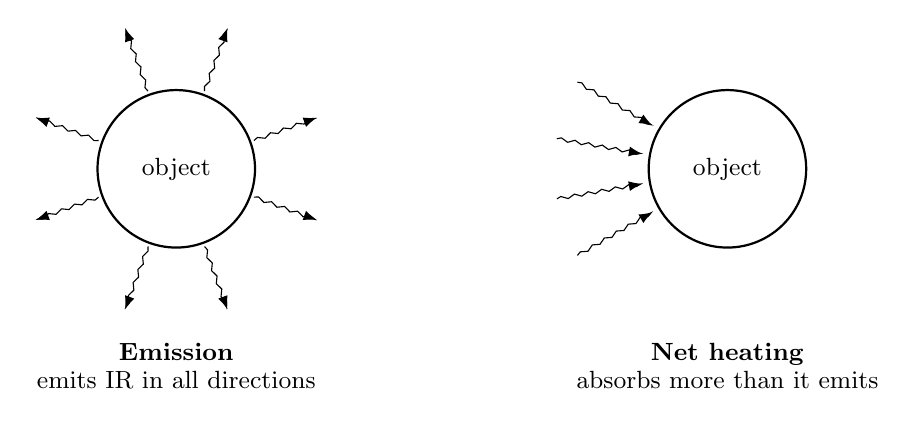
\begin{tikzpicture}[>=Latex]
% radiation balance diagram
\draw[thick] (0,0) circle (1.0);
\node at (0,0) {\small object};
% emission arrows outward
\foreach \a in {20,70,110,160,200,250,290,340}{
  \draw[->,decorate,decoration={snake,amplitude=0.6pt,segment length=5pt}]
    (\a:1.05) -- (\a:1.9);
}
\node[align=center] at (0,-2.5) {\small\textbf{Emission}\\[-2pt]\small emits IR in all directions};

% absorbing object
\begin{scope}[xshift=7cm]
\draw[thick] (0,0) circle (1.0);
\node at (0,0) {\small object};
\foreach \a in {150,170,190,210}{
  \draw[->,decorate,decoration={snake,amplitude=0.6pt,segment length=5pt}]
    (\a:2.2) -- (\a:1.1);
}
\node[align=center] at (0,-2.5) {\small\textbf{Net heating}\\[-2pt]\small absorbs more than it emits};
\end{scope}
\end{tikzpicture}
\end{center}

\begin{itemize}[leftmargin=1.4em,itemsep=1pt]
  \item A \textbf{cooling} object emits \emph{more} infrared than it absorbs.
  \item A \textbf{heating} object absorbs \emph{more} than it emits (it still emits some).
  \item At \textbf{thermal equilibrium} emission rate $=$ absorption rate, and the
        temperature is constant.
\end{itemize}

\subsubsection{Black/matt vs white/shiny surfaces}

\begin{keybox}[The two exam surfaces]
\begin{center}
\renewcommand{\arraystretch}{1.3}
\begin{tabular}{@{}p{4.5cm}p{4.7cm}p{4.7cm}@{}}
\toprule
\textbf{Surface} & \textbf{Emit / absorb} & \textbf{Reflect} \\
\midrule
Black, matt (dull, rough) & \textbf{Best} emitter and absorber & Poor reflector \\
White/light, shiny (mirror) & \textbf{Worst} emitter and absorber & \textbf{Best} reflector \\
\bottomrule
\end{tabular}
\end{center}
Good emitters are good absorbers --- these "go together." Reflection is the
\emph{opposite} of absorption. So a shiny surface, being the best reflector, is the
\emph{worst} emitter and absorber.
\end{keybox}

In the black-vs-shiny can demonstration, both cans hold hot water at the \emph{same}
temperature; the black can appears hotter on the infrared camera because it \emph{emits}
more infrared. When Phuc suggested the shiny (reflective) can should "give more," Alex
corrected the setup: reflection needs incoming radiation, but here the source is the hot
water \emph{inside}, so what matters is \emph{emission}, and black wins.

\begin{watchbox}
\textbf{Keep these three verbs surgically separate:}
\emph{emit} $=$ give off; \emph{absorb} $=$ take in; \emph{reflect} $=$ bounce back
incoming radiation. "Best reflector" and "best absorber" are \emph{opposites}, never the
same surface.
\end{watchbox}

\subsubsection{Global warming --- exactly as taught, corrected where needed}

The board explanation (Figure~\ref{fig:0109-05}) ran:
\begin{enumerate}[leftmargin=1.5em,itemsep=1pt]
  \item Infrared (and other radiation) is given off by the Sun and travels to Earth.
  \item Earth \textbf{absorbs} it and warms.
  \item Earth \textbf{re-emits} radiation at a \emph{different (longer-wavelength/lower)
        frequency}.
  \item Gases in the atmosphere (notably \textbf{CO\textsubscript{2}}) let the Sun's
        incoming radiation through but \emph{trap} much of the outgoing re-emitted
        radiation.
  \item For millions of years absorption and emission balanced (equilibrium). Added
        CO\textsubscript{2} traps more outgoing radiation, slowing the cooling and raising
        the temperature.
\end{enumerate}

\begin{plainbox}
\textbf{Physics tightening (textbook-correct).} The mechanism is sound as taught. To make
it exam-watertight: the Sun emits mostly \emph{short-wavelength} radiation (much of it
visible/near-infrared) which passes through the atmosphere; the warmed Earth re-emits
\emph{longer-wavelength infrared}; greenhouse gases (CO\textsubscript{2}, water vapour,
methane) absorb and re-radiate this outgoing infrared, reducing the rate at which energy
escapes. The Earth then settles at a \emph{higher} equilibrium temperature. Say
"different (longer) wavelength," not "the atmosphere knocks the radiation out."
\end{plainbox}

\begin{watchbox}
\textbf{Correction on the board (9 July \ts{27:11--29:09}).} Phuc called infrared "a weak
type of nuclear radiation." \textbf{Wrong.} "Radiation" broadly just means something is
given off. \emph{Nuclear} radiation is specifically \textbf{alpha, beta, gamma} from the
nucleus. Infrared and visible light are \emph{electromagnetic} radiation, emitted when an
orbital \emph{electron drops to a lower energy level and releases a photon} --- nothing to
do with the nucleus.
\end{watchbox}

\subsection{Conduction}

\subsubsection{In all solids: passing on vibrations}
\begin{defbox}[Conduction]
Heat transfer through a material (best in solids) by particles \textbf{passing on their
vibrations} to neighbouring particles, without the particles themselves moving along.
\end{defbox}

The board's formal sequence:
\begin{enumerate}[leftmargin=1.5em,itemsep=1pt]
  \item All particles vibrate all the time.
  \item Particles in the \emph{hotter} part of the solid vibrate \emph{more}.
  \item They pass these vibrations to neighbouring particles, which pass them on again ---
        energy travels toward the cooler end.
\end{enumerate}
Alex's analogy: people linking arms; one shakes, the next shakes, and so on down the line.

\subsubsection{Why metals are best: free electrons}
\begin{keybox}[Metals conduct best because\ldots]
\ldots they contain \textbf{free (delocalised) electrons}. These are knocked by the
vibrating atoms, move rapidly through the lattice and collide with atoms further along,
transferring energy \emph{much faster} than vibration-passing alone.
\end{keybox}

\begin{center}
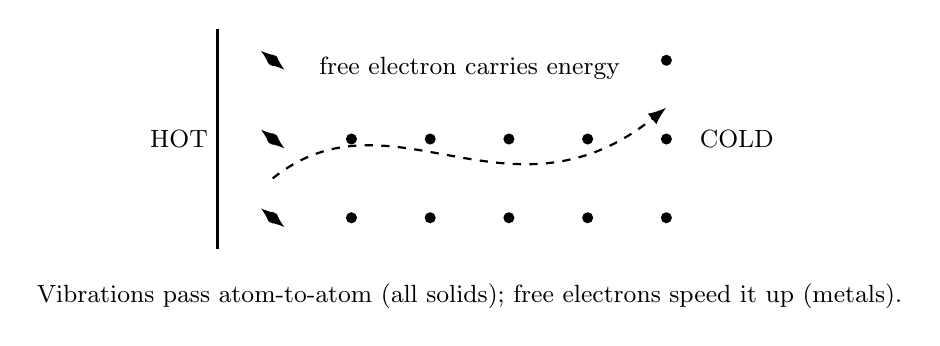
\begin{tikzpicture}[>=Latex]
% lattice of atoms
\foreach \x in {0,1,2,3,4,5}{
  \foreach \y in {0,1,2}{
    \fill (\x,\y) circle (2pt);
  }
}
% heat source left
\draw[thick] (-0.7,-0.4) -- (-0.7,2.4);
\node[left] at (-0.7,1.0) {\small HOT};
\node[right] at (5.3,1.0) {\small COLD};
% free electron path
\draw[->,thick,dashed] (0,0.5) .. controls (1.5,1.7) and (3,-0.2) .. (5,1.4);
\node[fill=white] at (2.5,1.9) {\small free electron carries energy};
% vibration arrows near hot end
\foreach \y in {0,1,2}{
  \draw[<->] (-0.15,\y+0.12) -- (0.15,\y-0.12);
}
\node[align=center] at (2.5,-1.0)
  {\small Vibrations pass atom-to-atom (all solids); free electrons speed it up (metals).};
\end{tikzpicture}
\end{center}

\subsubsection{Thermal vs electrical conduction}
They are related but distinct. In \emph{electrical} conduction the free electrons drift in
an \emph{organised} direction under an electric field/potential difference. In
\emph{thermal} conduction energy spreads via lattice vibrations and less-directed electron
motion from hot toward cold. The same free electrons make good electrical conductors also
good thermal conductors.

\begin{watchbox}
\textbf{Melting-ice demo (9 July \ts{37:05--40:12}).} Two blocks in the same room, both at
$\sim$\SI{21}{\celsius}, different materials; identical ice on each. The ice on block~2
melts in $\sim$\SI{12}{s}; the ice on block~1 barely melts. \textbf{Same temperature} ---
so it is not that one block is "hot." Block~2 is simply a \textbf{better thermal
conductor}: it transfers energy to the ice by contact much faster. Phuc's first answer
("the surface must be hot") was corrected on exactly this point.
\end{watchbox}

\subsection{Convection}

\begin{defbox}[Convection]
Heat transfer in \textbf{fluids} (liquids or gases) in which the heated fluid itself
physically \emph{moves}, carrying its energy with it.
\end{defbox}

\begin{keybox}[The convection chain --- say it in order]
Heated part of the fluid: particles \textbf{gain energy} $\to$ \textbf{move faster} $\to$
\textbf{spread apart} $\to$ that region becomes \textbf{less dense} $\to$ it \textbf{rises}.
Cooler fluid: particles move less $\to$ come closer $\to$ region becomes \textbf{more
dense} $\to$ it \textbf{sinks} to replace the risen fluid. The circulating flow is a
\textbf{convection current}.
\end{keybox}

\begin{center}
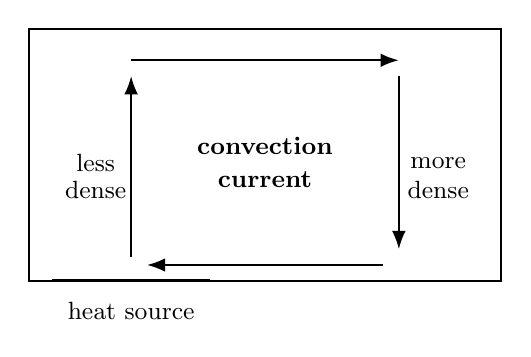
\begin{tikzpicture}[>=Latex]
\draw[thick] (0,0) rectangle (6,3.2);
% heater bottom-left
\draw[line width=1.2pt] (0.3,0) -- (2.3,0);
\node[below] at (1.3,-0.15) {\small heat source};
% circulation arrows
\draw[->,thick] (1.3,0.3) -- (1.3,2.6); % rise on left
\draw[->,thick] (1.3,2.8) -- (4.7,2.8); % across top
\draw[->,thick] (4.7,2.6) -- (4.7,0.4); % sink on right
\draw[->,thick] (4.5,0.2) -- (1.5,0.2); % back along bottom
\node at (0.85,1.5) {\small less};
\node at (0.85,1.15) {\small dense};
\node at (5.2,1.5) {\small more};
\node at (5.2,1.15) {\small dense};
\node[align=center] at (3,1.5) {\small\textbf{convection}\\\small\textbf{current}};
\end{tikzpicture}
\end{center}

\begin{watchbox}
\textbf{Density, not size (Alex's nightclub analogy).} When a fluid is heated the particles
do \emph{not} get bigger --- they \emph{spread out}, so the same mass occupies more volume
and the density falls. Think of a dance floor: an energetic song makes people move more and
spread out, lowering the crowd density.
\end{watchbox}

\textbf{Land/sea breeze (daytime).} The Sun heats the \emph{land} by infrared; land warms
faster than the sea and heats the air above it. That air rises (less dense); cooler air
over the sea moves in to replace it --- a sea breeze, a convection current.

\begin{watchbox}
\textbf{Two convection corrections to Phuc.} (i) Cooling air does \emph{not} have to turn
to liquid to sink --- a gas can just become denser and sink while staying a gas. (ii) In
the dyed-water loop, the water is \emph{not} heated enough to change state; it stays liquid
and the dye simply reveals the circulating current.
\end{watchbox}

\subsection{Insulation --- controlling all three mechanisms}

The unifying idea: \textbf{trapped air}. Air has few particles (poor conductor) and, when
trapped in small pockets, cannot circulate (no convection). A vacuum is even better for
conduction (no particles at all), and shiny/foil surfaces defeat radiation.

\begin{center}
\renewcommand{\arraystretch}{1.3}
\begin{tabular}{@{}p{4.6cm}p{4.4cm}p{5.2cm}@{}}
\toprule
\textbf{Feature} & \textbf{Mechanism reduced} & \textbf{Why} \\
\midrule
Loft insulation (thick fibre roll) & Conduction \emph{and} convection & Trapped air
conducts poorly; pockets stop air circulating. \\
Cavity-wall insulation & Conduction \emph{and} convection & Fibres between two brick
layers trap air; stops warm air flowing through the cavity. \\
Double / triple glazing & Conduction & Air (or argon) gap between panes is a poor
conductor. \\
Draught excluder & Convection & Blocks whole volumes of hot/cold air flowing under doors. \\
Curtains / blinds & Conduction (and some convection) & Trap a layer of air like a cavity
wall. \\
Silver reflective cover / foil behind radiator & Radiation & Reflects infrared back;
poor emitter. \\
Vacuum (ideal) & Conduction \emph{and} convection & No particles $\Rightarrow$ neither
process can occur. \\
\bottomrule
\end{tabular}
\end{center}

\begin{center}
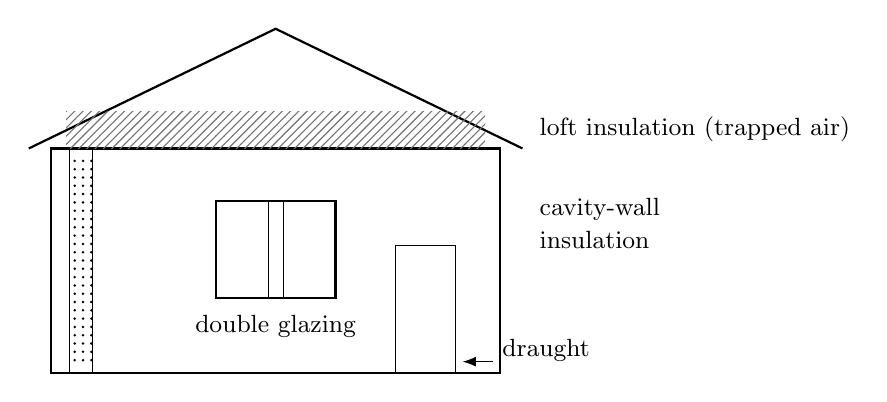
\begin{tikzpicture}[>=Latex,scale=0.95]
% simple house cross-section
\draw[thick] (0,0) rectangle (6,3);
\draw[thick] (-0.3,3) -- (3,4.6) -- (6.3,3); % roof
% loft insulation hatch
\fill[pattern=north east lines, pattern color=guidegrey] (0.2,3) rectangle (5.8,3.5);
\node[right] at (6.4,3.25) {\small loft insulation (trapped air)};
% cavity wall
\draw (0.25,0)--(0.25,3); \draw (0.55,0)--(0.55,3);
\fill[pattern=dots] (0.25,0.1) rectangle (0.55,2.9);
\node[align=left,right] at (6.4,2.0) {\small cavity-wall\\\small insulation};
% window with double glazing
\draw[thick] (2.2,1)--(3.8,1)--(3.8,2.3)--(2.2,2.3)--cycle;
\draw (2.9,1)--(2.9,2.3); \draw (3.1,1)--(3.1,2.3);
\node[below] at (3,0.9) {\small double glazing};
% door + draught
\draw (4.6,0)--(4.6,1.7)--(5.4,1.7)--(5.4,0);
\draw[->] (5.9,0.15)--(5.5,0.15);
\node[right] at (5.9,0.3) {\small draught};
\end{tikzpicture}
\end{center}

\begin{watchbox}
\textbf{Draught correction (10 July \ts{18:56--20:22}).} A draught is \textbf{convection},
not conduction: whole volumes of hot and cold air flow and replace one another. Phuc first
answered "conduction"; the give-away is \emph{moving/replacing air}.
\end{watchbox}

\subsection{Specific heat capacity (SHC)}

\begin{defbox}[Specific heat capacity]
The energy needed to raise the temperature of \textbf{\SI{1}{\kilogram}} of a substance by
\textbf{\SI{1}{\kelvin}} (equivalently \SI{1}{\celsius}). Symbol $c$, unit
\si{\joule\per\kilogram\per\kelvin}.
\end{defbox}

\[
\boxed{\;\dE = mc\,\dtheta\;}
\qquad\Longrightarrow\qquad
c = \frac{\dE}{m\,\dtheta}
\]

\begin{center}
\renewcommand{\arraystretch}{1.3}
\begin{tabular}{@{}llll@{}}
\toprule
\textbf{Symbol} & \textbf{Quantity} & \textbf{Unit} & \textbf{Note} \\
\midrule
$\dE$ & energy transferred & \si{\joule} & \\
$m$ & mass & \si{\kilogram} & always convert grams to kg \\
$c$ & specific heat capacity & \si{\joule\per\kilogram\per\kelvin} & always given in the exam \\
$\dtheta$ & temperature change & \si{\kelvin} or \si{\celsius} & interval is identical in both \\
\bottomrule
\end{tabular}
\end{center}

Because a \SI{1}{\kelvin} interval equals a \SI{1}{\celsius} interval, $\dtheta$ may be
quoted in either; the SHC unit is written \si{\joule\per\kilogram\per\kelvin} or
\si{\joule\per\kilogram\per\celsius}. Reference value: water $c = \SI{4200}{\joule\per\kilogram\per\kelvin}$
(unusually high --- why water is good for radiators and slow to heat/cool).

\subsubsection{Measuring $c$ (the aluminium-block practical)}
Electrical energy supplied $=$ increase in internal energy of the block:
\[
IV\,\Delta t = mc\,(\theta_f - \theta_i)
\qquad\Longrightarrow\qquad
c = \frac{IV\,\Delta t}{m(\theta_f-\theta_i)} .
\]
\textbf{Method (Core-Practical style).} Weigh a \SI{1}{\kilogram} aluminium block; insert a
heater and thermometer (a little oil in the holes for good thermal contact); record
starting temperature; switch on and record $I$, $V$ and time; after a set time record the
highest steady temperature; compute $c$.

\begin{keybox}[Why the measured $c$ comes out too large --- know these errors]
\begin{itemize}[leftmargin=1.4em,itemsep=1pt]
  \item Energy is absorbed by the \emph{heater itself} (main error) --- not all supplied
        energy heats the block.
  \item Energy is \emph{lost to the surroundings} despite lagging.
  \item A little energy is taken by the \emph{lagging and thermometer}.
  \item Thermometer/meter inaccuracies (small $\dtheta$ worsens this).
\end{itemize}
All of the first three mean the block gets \emph{less} energy than you counted, so the
calculated $c = \dE/(m\dtheta)$ is \textbf{too large}.
\end{keybox}

\subsection{Specific latent heat}

\begin{defbox}[Specific latent heat]
The energy needed to change the state of \textbf{\SI{1}{\kilogram}} of a substance
\emph{with no change in temperature}. Symbol $L$, unit \si{\joule\per\kilogram}.
\begin{itemize}[leftmargin=1.3em,itemsep=0pt]
  \item \textbf{Fusion} ($L_f$): solid $\leftrightarrow$ liquid (melting/freezing).
  \item \textbf{Vaporisation} ($L_v$): liquid $\leftrightarrow$ gas (boiling/condensing).
\end{itemize}
\end{defbox}

\[
\boxed{\;\dE = L\,\Delta m\;}
\]

During a change of state, energy goes into \emph{potential} energy (breaking/loosening
bonds), not kinetic energy --- so the temperature stays constant while the state changes.
For water, $L_f = \SI{3.34e5}{\joule\per\kilogram}$ and
$L_v = \SI{2.26e6}{\joule\per\kilogram}$: vaporisation needs roughly \emph{seven times}
more energy than fusion, because boiling must \emph{fully separate} the molecules, whereas
melting only lets them slide past one another.

\subsubsection{The heating curve}
\begin{center}
\begin{tikzpicture}
\begin{axis}[
  width=12cm, height=6.2cm,
  xlabel={energy supplied}, ylabel={temperature},
  xtick=\empty, ytick=\empty,
  xmin=0,xmax=10, ymin=0,ymax=6,
  axis lines=left, clip=false]
% solid heating
\addplot[thick] coordinates {(0,1)(2,2.5)};
% melting plateau
\addplot[thick] coordinates {(2,2.5)(4,2.5)};
% liquid heating
\addplot[thick] coordinates {(4,2.5)(6,4.3)};
% boiling plateau
\addplot[thick] coordinates {(6,4.3)(9,4.3)};
\node[anchor=south] at (axis cs:1,1.7) {\scriptsize solid};
\node[anchor=south] at (axis cs:3,2.5) {\scriptsize melting ($L_f$)};
\node[anchor=south] at (axis cs:5,3.3) {\scriptsize liquid};
\node[anchor=south] at (axis cs:7.5,4.3) {\scriptsize boiling ($L_v$)};
\draw[dashed] (axis cs:2,0)--(axis cs:2,2.5);
\draw[dashed] (axis cs:6,0)--(axis cs:6,4.3);
\end{axis}
\end{tikzpicture}
\end{center}
The \textbf{sloped} sections are $\dE = mc\,\dtheta$ (temperature rising, one state). The
\textbf{flat plateaus} are $\dE = L\,\Delta m$ (state changing, temperature constant); the
boiling plateau is much longer than the melting plateau because $L_v \gg L_f$.

\subsection{Fixed-volume gas pressure and gas-law context}

The particle explanation of fixed-volume pressure was covered in
Section~\ref{sec:fixedgas-warmup}. Formalised for Unit~5:

\begin{keybox}[Pressure of a fixed mass of gas]
\textbf{Pressure law (constant volume):} $p \propto T$, i.e.
$\dfrac{p_1}{T_1} = \dfrac{p_2}{T_2}$ with $T$ in \textbf{kelvin}.

\smallskip
\textbf{Kinetic-theory picture:} heating $\to$ particles faster $\to$ more frequent, harder
wall collisions $\to$ greater force on a fixed wall area $\to$ higher pressure.

\smallskip
\textbf{Ideal gas equation:} $pV = NkT$ with $k = \SI{1.38e-23}{\joule\per\kelvin}$.
\textbf{Boyle's law} (constant $T$): $p_1V_1 = p_2V_2$.
\end{keybox}

\begin{center}
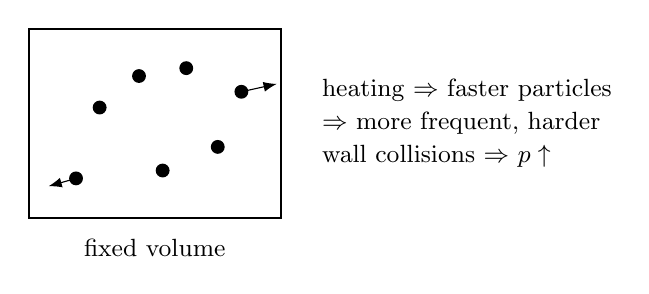
\begin{tikzpicture}[>=Latex]
\draw[thick] (0,0) rectangle (3.2,2.4);
% place particles deterministically
\foreach \p in {(0.6,0.5),(1.4,1.8),(2.4,0.9),(0.9,1.4),(2.0,1.9),(2.7,1.6),(1.7,0.6)}{
  \fill \p circle (2.5pt);
}
% collision arrows on walls
\draw[->] (2.7,1.6)--(3.15,1.7);
\draw[->] (0.6,0.5)--(0.25,0.4);
\node[below] at (1.6,-0.15) {\small fixed volume};
\node[right,align=left] at (3.6,1.2)
  {\small heating $\Rightarrow$ faster particles\\\small $\Rightarrow$ more frequent, harder\\\small wall collisions $\Rightarrow$ $p\uparrow$};
\end{tikzpicture}
\end{center}

The mean molecular kinetic energy links directly to temperature:
\[
\tfrac{1}{2}m\langle c^2\rangle = \tfrac{3}{2}kT ,
\]
so the average random kinetic energy of gas molecules is proportional to the
\emph{absolute} temperature --- and would be zero at \SI{0}{K}.

\subsection{Heat transfer in space --- why a vacuum does not cool a machine}

\begin{keybox}[Space cooling from first principles]
In a \textbf{vacuum} there are no particles, so:
\begin{itemize}[leftmargin=1.4em,itemsep=1pt]
  \item \textbf{No conduction} --- nothing to pass vibrations to.
  \item \textbf{No convection} --- no fluid to circulate.
  \item \textbf{Only radiation} --- a body can lose heat solely by \emph{emitting
        infrared}.
\end{itemize}
So a hot machine in space is \emph{not} automatically cooled by "cold" space. It can only
reject heat by \textbf{radiative cooling}.
\end{keybox}

The engineering answer Alex built with Phuc: conduct the internal heat to a
\textbf{large, matte-black radiator} (a good emitter, large area) that radiates infrared to
space; and add a \textbf{reflective (silver) layer} facing the Sun to reflect incoming
solar radiation so it is not absorbed. A radiator made \emph{large enough} can emit both
the internally generated heat and the absorbed solar input. This is exactly why spacecraft
and astronauts carry reflective outer layers plus dedicated radiator panels. (Illustrative
figures used: solar input $\sim\SI{1000}{\watt\per\metre\squared}$, internal generation
$\sim500$ in the same illustrative units --- the emitter must handle their sum.)

\clearpage
% ===========================================================================
\section{Every recoverable exercise and question}
\label{sec:exercises}
% ===========================================================================

Each item gives the exact board prompt and visible values, the reasoning, the answer,
Phuc's evidenced response and Alex's correction, and exam technique. The relevant
screenshot is placed near the question.

% --------- Q group A: 9 July retrieval ---------
\subsection{9 July opening retrieval}

\begin{figure}[h]
\centering
\includegraphics[width=0.82\textwidth]{\imgA{01_00_image.png}}
\caption{9 July, screenshot 01 --- opening retrieval board. \textsc{thermal} (a store) is
circled and linked to \textsc{heating} (a transfer) to force the store-vs-pathway
distinction.}
\label{fig:0109-01}
\end{figure}

\begin{figure}[h]
\centering
\includegraphics[width=0.82\textwidth]{\imgA{02_00_image.png}}
\caption{9 July, screenshot 02 --- completed opening retrieval, including the fixed-volume
gas reasoning ($p\uparrow$ because faster, frequent wall collisions, force $\uparrow$,
$p=F/A$).}
\label{fig:0109-02}
\end{figure}

\begin{enumerate}[leftmargin=1.6em,itemsep=4pt,label=\textbf{A\arabic*.}]
\item \textbf{List the energy stores.} \\
  \emph{Answer (board):} KE, GPE, elastic, chemical, \textbf{thermal}, nuclear,
  (electro)magnetic. \\
  \emph{Phuc:} gave KE, potential (refined to GPE), elastic, chemical; asked "are there
  only five?" \emph{Alex:} "a few more" --- and admits nobody reliably remembers the full
  list. Focus falls on the \emph{thermal} store.

\item \textbf{List the energy transfers.} \\
  \emph{Answer:} heating; electrically; radiation (waves --- light, sound); mechanically
  (force $\times$ distance). \\
  \emph{Technique:} keep this list separate from the stores list.

\item \textbf{List some hot objects.} \\
  \emph{Answer (board, in red):} Sun, engine, oven. Used repeatedly as "more infrared"
  comparators.

\item \textbf{State what everything is made up of.} \emph{Answer:} atoms (particles).

\item \textbf{Explain what happens to the pressure of a fixed volume of gas as it is
  heated.} \\
  Worked in full in Section~\ref{sec:fixedgas-warmup}. \emph{Answer:} pressure rises
  (faster particles $\to$ more frequent, harder wall collisions $\to$ greater force on a
  fixed area $\to$ $p\uparrow$). \emph{Phuc's slips:} "expands," "more friction into the
  boxes," "mass $\div$ volume" --- all corrected.
\end{enumerate}

% --------- Q group: IR climate ---------
\subsection{Infrared and the Sun--Earth question}

\begin{figure}[h]
\centering
\includegraphics[width=0.55\textwidth]{\imgA{03_00_image.png}}\hfill
\includegraphics[width=0.42\textwidth]{\imgA{04_00_image.png}}
\caption{9 July, screenshots 03 and 04 --- infrared emission/absorption rules (left) and
the emitter/absorber comparison (right), where "best reflector" is crossed out beside the
shiny can and black/matt is labelled best emitter/absorber.}
\label{fig:0109-0304}
\end{figure}

\begin{figure}[h]
\centering
\includegraphics[width=0.72\textwidth]{\imgA{03_01_image.png}}
\caption{9 July, screenshot 03\_01 --- thermal-camera evidence contrasting the shiny and
black/matt surfaces at the same temperature: the black/matt surface shows up as the stronger
infrared emitter.}
\label{fig:0109-0301}
\end{figure}

\begin{figure}[h]
\centering
\includegraphics[width=0.82\textwidth]{\imgA{05_00_image.png}}
\caption{9 July, screenshot 05 --- "How does heat get from the Sun to Earth?" with the
five-step trapping explanation and CO\textsubscript{2}/atmosphere labels.}
\label{fig:0109-05}
\end{figure}

\begin{enumerate}[leftmargin=1.6em,itemsep=4pt,label=\textbf{B\arabic*.}]
\item \textbf{How does heat get from the Sun to Earth, and why is Earth heating up?} \\
  \emph{Answer:} the Sun emits infrared/radiation $\to$ Earth absorbs it $\to$ Earth
  re-emits at a different (longer) frequency $\to$ CO\textsubscript{2}/atmosphere traps
  more of the outgoing radiation $\to$ the balance shifts and Earth warms. \\
  \emph{Phuc's misconception:} "infrared is a weak type of nuclear radiation."
  \emph{Correction:} infrared is electromagnetic (electron energy-level drops), not
  alpha/beta/gamma from the nucleus. \\
  \emph{Technique:} name the re-emission at a \emph{different wavelength} explicitly ---
  it is the crux of the greenhouse argument.

\item \textbf{Which can emits more infrared (black vs shiny, same hot water inside)?} \\
  \emph{Answer:} the \textbf{black/matt} can --- best emitter. \emph{Phuc:} thought the
  shiny reflector should "give more"; corrected --- reflection needs an external source,
  but the source here is internal, so emission (black) wins.
\end{enumerate}

% --------- Cooling curve ---------
\subsection{Black-vs-silver cooling curve}

\begin{plainbox}
\textbf{Experiment.} Black and silver cans, \emph{same} volume of hot water at the
\emph{same} start temperature ($\sim$\SI{80}{\celsius} illustrative). Record temperature
every \SI{30}{s}; plot temperature against time.

\smallskip
\textbf{Question:} how do you know the black can emits more infrared? \\
\textbf{Answer:} its cooling curve \emph{falls faster} --- it loses energy more quickly.
\end{plainbox}

\begin{center}
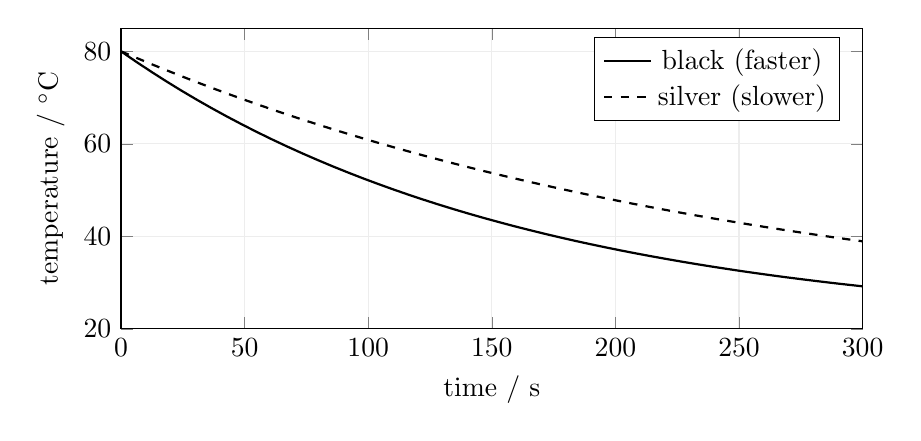
\begin{tikzpicture}
\begin{axis}[width=11cm,height=5.4cm,xlabel={time / s},ylabel={temperature / \si{\celsius}},
  xmin=0,xmax=300,ymin=20,ymax=85, legend pos=north east, grid=both,
  grid style={lightgrey}, samples=50]
\addplot[thick,domain=0:300]{20+60*exp(-x/160)};
\addlegendentry{black (faster)}
\addplot[thick,dashed,domain=0:300]{20+60*exp(-x/260)};
\addlegendentry{silver (slower)}
\end{axis}
\end{tikzpicture}
\end{center}

\begin{watchbox}
\textbf{Phuc's slip (9 July \ts{33:25--34:44}).} He predicted the strong emitter's
temperature would become \emph{higher}. \textbf{Wrong:} giving off energy makes an object
\emph{cool down}. Read emission from the \emph{rate of cooling}, never from a claim that
the emitter gets hotter.
\end{watchbox}

% --------- Conduction ---------
\subsection{Conduction demonstrations}

\begin{figure}[h]
\centering
\includegraphics[width=0.62\textwidth]{\imgA{06_00_image.png}}\hfill
\includegraphics[width=0.35\textwidth]{\imgA{07_00_image.png}}
\caption{9 July, screenshots 06 and 07 --- melting-ice conduction demo (both blocks at
\SI{21}{\celsius}; block~2 is the good conductor) and the microscopic conduction/free-electron
diagram.}
\label{fig:0109-0607}
\end{figure}

\begin{enumerate}[leftmargin=1.6em,itemsep=4pt,label=\textbf{C\arabic*.}]
\item \textbf{Which block melts the ice first?} (Both at \SI{21}{\celsius}, different
  materials.) \\
  \emph{Answer:} block~2 --- it transfers energy to the ice quickly, so it is the
  \textbf{good conductor}. \emph{Phuc:} first said the block "must be hot"; corrected
  --- both are at the same temperature, the difference is \emph{conductivity}.
\item \textbf{Metal-rod-and-wax: which attached piece falls first?} \\
  \emph{Answer:} the piece \emph{nearest the heated end}, then successively outward as
  energy travels along the rod. \emph{Reasoning:} vibrations (and free-electron transfer)
  carry energy from the hot end outward.
\item \textbf{Fill-ins: best insulator / good insulators.} \\
  \emph{Answers (board):} best insulator $=$ \textbf{vacuum}; good insulators $=$
  \textbf{gas / air}. \emph{Phuc's slip:} suggested "very strong chemical bonds" make the
  best insulator --- corrected: strong bonds \emph{transmit} vibration; \emph{weaker}
  bonds and \emph{fewer/no} particles reduce conduction.
\end{enumerate}

\begin{figure}[h]
\centering
\includegraphics[width=0.80\textwidth]{\imgA{08_00_image.png}}
\caption{9 July, screenshot 08 --- the conduction sequence board, ending on the insulation
ranking: a \emph{vacuum} (no particles) is the best insulator and \emph{gas/air} (few, widely
spaced particles) a good insulator.}
\label{fig:0109-08}
\end{figure}

% --------- Convection ---------
\subsection{Convection demonstrations}

\begin{figure}[h]
\centering
\includegraphics[width=0.60\textwidth]{\imgA{09_00_image.png}}\hfill
\includegraphics[width=0.37\textwidth]{\imgA{10_00_image.png}}
\caption{9 July, screenshots 09 and 10 --- the five-step convection sequence with the
daytime sea-breeze diagram (left) and the practical/demo board: heated dyed-water loop,
candle-and-smoke box, warm/cold bottles (right).}
\label{fig:0109-0910}
\end{figure}

\begin{enumerate}[leftmargin=1.6em,itemsep=4pt,label=\textbf{D\arabic*.}]
\item \textbf{Dyed-water loop: what happens when one corner is heated?} \\
  \emph{Answer:} particles in the heated region move faster, spread out, become less
  dense and rise; fluid on the other side sinks; the dye circulates, revealing the
  convection current. \emph{Phuc's slips:} thought the water might boil/"become gas," and
  that it might "drop" --- corrected: not heated enough to change state; heated fluid
  \emph{rises}.
\item \textbf{Candle-and-smoke box (two openings).} \\
  \emph{Answer:} hot air rises over the flame; smoke is drawn down the other opening ---
  a visible convection current.
\end{enumerate}

\begin{figure}[h]
\centering
\includegraphics[width=0.80\textwidth]{\imgA{11_00_image.png}}
\caption{9 July, screenshot 11 --- end-of-lesson retrieval: conduction, infrared radiation,
convection, free electrons, insulator.}
\label{fig:0109-11}
\end{figure}

\subsection{9 July end-of-lesson retrieval}
\begin{enumerate}[leftmargin=1.6em,itemsep=2pt,label=\textbf{E\arabic*.}]
\item Heat transfer through collision of particles $=$ \textbf{conduction}. \emph{(Phuc: correct.)}
\item Heat transfer via electromagnetic waves $=$ \textbf{infrared radiation}. \emph{(Phuc
  said "infrared light"; Alex preferred "radiation.")}
\item Heat transfer by movement of less-dense fluids $=$ \textbf{convection}. \emph{(Phuc
  needed the prompt.)}
\item Metals are best conductors because $=$ \textbf{free electrons}. \emph{(Correct,
  praised.)}
\item The opposite of a good conductor is a good $=$ \textbf{insulator}.
\end{enumerate}

% --------- 10 July house exercise ---------
\subsection{10 July: retrieval and the house-insulation exercise}

\begin{figure}[h]
\centering
\includegraphics[width=0.80\textwidth]{\imgB{01_00_image.png}}
\caption{10 July, screenshot 01 --- repeat retrieval (conduction, infrared radiation,
convection, free electrons, insulator) with ticks and a struck-through item.}
\label{fig:0110-01}
\end{figure}

\begin{figure}[h]
\centering
\includegraphics[width=0.80\textwidth]{\imgB{02_00_image.png}}
\caption{10 July, screenshot 02 --- the house-insulation exercise in progress: the labelled
house outline before the printed answer block is worked through.}
\label{fig:0110-02}
\end{figure}

\begin{figure}[h]
\centering
\includegraphics[width=0.80\textwidth]{\imgB{04_00_image.png}}
\caption{10 July, screenshot 04 --- completed house-insulation exercise with the printed
answer block (double glazing, cavity-wall insulation, roof insulation, draught excluders,
foil behind radiator) and added draught/gap annotations.}
\label{fig:0110-04}
\end{figure}

\begin{plainbox}
\textbf{Exercise prompt.} "Add labels to the house to suggest methods of insulation, and
explain which of the three methods of heat transfer they help to reduce."

\smallskip
\textbf{Board answer block (exact):}
\begin{enumerate}[leftmargin=1.6em,itemsep=1pt]
  \item \textbf{Double glazing} --- reduces \emph{conduction}, because there is a layer of
        air trapped between two panes of glass; air is a poor conductor.
  \item \textbf{Cavity-wall insulation} (glass fibres filling the gap between inner and
        outer wall) --- reduces \emph{convection}, because the fibres stop warm air flowing
        through the cavity.
  \item \textbf{Roof (loft) insulation} --- as above (reduces conduction and convection).
  \item \textbf{Draught excluders} --- reduce \emph{convection}, because they stop
        draughts of air escaping under doors.
  \item \textbf{Foil layer behind radiator} --- reflects \emph{infrared radiation} back
        into the room.
\end{enumerate}
\end{plainbox}

\begin{watchbox}
\textbf{Draught mechanism.} When Alex asked whether a draught (flowing air) is conduction,
convection or radiation, Phuc answered \emph{conduction} --- corrected to
\textbf{convection} (whole volumes of air move and are replaced).
\end{watchbox}

% --------- Sahara-Paris ---------
\subsection{10 July: the Sahara-to-Paris heatwave model}

\begin{figure}[h]
\centering
\includegraphics[width=0.86\textwidth]{\imgB{03_00_image.png}}
\caption{10 July, screenshot 03 --- the Paris/Sahara heatwave sketch, with illustrative
temperatures (\SI{30}{}, \SI{40}{}, \SI{50}{}, \SI{60}{\celsius}), "IR from Sun" arrows and
"air conduction" at the surface.}
\label{fig:0110-03}
\end{figure}

\begin{plainbox}
\textbf{Question.} Why does the outdoor air get so hot in a heatwave --- is it radiation or
convection? \\
\textbf{Answer: a combination of all three mechanisms.}
\begin{enumerate}[leftmargin=1.6em,itemsep=1pt]
  \item The Sahara ground is heated by the Sun's \textbf{infrared}.
  \item Air just above the hot sand is heated by \textbf{conduction} from the ground
        (passing vibrations).
  \item That hot air becomes less dense, rises, and is transported toward Paris by
        large-scale \textbf{convection}.
  \item Locally, infrared heats the streets and the Eiffel Tower, and those hot solids
        reheat the nearby air by conduction.
\end{enumerate}
\emph{Illustrative arithmetic (Alex's, explicitly "made-up"):} air leaves the Sahara at
$\sim$\SI{60}{\celsius}, cools through \SI{50}{}, \SI{40}{}, arriving Paris at
$\sim$\SI{30}{\celsius}; local heating then adds $\sim$\SI{10}{\celsius} to
$\sim$\SI{40}{\celsius} at street level. These numbers are \emph{explanatory only}, not
data.
\end{plainbox}

\begin{watchbox}
\textbf{Phuc's either/or slip.} He asked whether the hot air was "not infrared but
convection." Corrected: it is \emph{both}, plus conduction --- do not force a single
mechanism when a real scenario combines them. (He also predicted clouds; Alex ruled clouds
out of scope here --- only air temperature matters.)
\end{watchbox}

% --------- SHC / latent heat calcs ---------
\subsection{10 July: specific heat capacity and the avocado calculations}

\begin{figure}[h]
\centering
\includegraphics[width=0.80\textwidth]{\imgB{05_00_image.png}}
\caption{10 July, screenshot 05 --- SHC definition, the $E=mc\Delta\theta$ / units map, the
water value \SI{4200}{\joule\per\kilogram\per\celsius}, and the copper-block question.}
\label{fig:0110-05}
\end{figure}

\begin{figure}[h]
\centering
\includegraphics[width=0.62\textwidth]{\imgB{06_00_image.png}}\hfill
\includegraphics[width=0.35\textwidth]{\imgB{07_00_image.png}}
\caption{10 July, screenshots 06 and 07 --- the SHC practical (water and aluminium, with
$E=mc\Delta\theta$ rearranged for $c$) and the avocado questions 3 and 4.}
\label{fig:0110-0607}
\end{figure}

\subsubsection*{Board example --- copper block (screenshot 05)}
\begin{plainbox}
\textbf{Prompt.} "A copper block has a specific heat capacity of
\SI{3850}{\joule\per\kilogram\per\kelvin}. It has a mass of \SI{0.5}{\kilogram} and is
heated by \SI{3}{\kelvin}. How much energy is transferred to the copper block?"

\smallskip
\textbf{Solution.}
\[
\dE = mc\,\dtheta = 0.5 \times 3850 \times 3 = \boxed{\SI{5775}{\joule}} .
\]
\end{plainbox}
\begin{watchbox}
\textbf{Board slip to avoid (screenshot 05).} The handwritten working copied the SHC as
"385" (dropping a zero from \textbf{3850}) and started to label the unknown with a
$\theta$-like symbol although the question asks for \emph{energy}, $E$. Copy values exactly
and write the correct target symbol.
\end{watchbox}

\subsubsection*{Board question 3 --- avocado SHC (screenshot 07)}
\begin{plainbox}
\textbf{Prompt (exact).} "What is the specific heat capacity of an avocado? An average
avocado has a mass of \SI{0.215}{\kilogram} and it takes \SI{1294}{\joule} for it to be
cooled down by \SI{2}{\kelvin}."

\smallskip
\textbf{Solution.} Rearrange $\dE = mc\,\dtheta$:
\[
c = \frac{\dE}{m\,\dtheta} = \frac{1294}{0.215 \times 2}
  = \frac{1294}{0.43} = \boxed{\SI{3009}{\joule\per\kilogram\per\kelvin}}
  \;(\text{to 4 s.f. } 3009.3).
\]
\end{plainbox}

\begin{watchbox}
\textbf{Important correction to the board answer.} The board circled
"$= \SI{2500}{\joule\per\kilogram\per\kelvin}$," but that does \emph{not} follow from the
numbers written. Using the board's own substitution,
$1294 \div (0.215 \times 2) = 1294 \div 0.43 = \mathbf{3009}$
(\si{\joule\per\kilogram\per\kelvin}), \emph{not} 2500. The \SI{2500}{} value traces to a
separate "let's make up a number, $1300 \div 0.5$" aside in the lesson --- and even that
was mis-stated aloud ($1300 \div 0.5 = 2600$, not 2500). \textbf{Use \SI{3009}{}} for the
avocado as printed. \emph{Lesson:} always re-key the division; a circled answer can still
be wrong.
\end{watchbox}

\subsubsection*{Board question 4 --- avocado temperature change (screenshot 07)}
\begin{plainbox}
\textbf{Prompt (exact).} "What is the change in temperature of an avocado of mass
\SI{0.215}{\kilogram} that gains \SI{3000}{\joule} of thermal energy?"

\smallskip
\textbf{Solution.} Use the $c$ from Q3 ($c = \SI{3009}{\joule\per\kilogram\per\kelvin}$) and
rearrange $\dE = mc\,\dtheta$ for $\dtheta$:
\[
\dtheta = \frac{\dE}{mc} = \frac{3000}{0.215 \times 3009}
  = \frac{3000}{646.9} = \boxed{\SI{4.64}{\kelvin}}\ (\approx \SI{4.6}{\kelvin}).
\]
\emph{(The board left Q4 unfinished at "$c=$"; this is the intended completion. If instead
you used the board's circled $c=\SI{2500}{}$, you would get
$\dtheta = 3000/(0.215\times2500) = \SI{5.58}{\kelvin}$ --- another reason to fix Q3
first.)}
\end{plainbox}

\subsection{Data note on the "Q3/Q4" spoken values}
The lesson audio around the calculations was partly garbled (a "1,294" energy, a made-up
"$1300 \div 0.5$," a spoken "2,500", an "avocado" follow-up). The \emph{screenshots}
resolve the exact printed questions (mass \SI{0.215}{\kilogram}, \SI{1294}{\joule},
\SI{2}{\kelvin} for Q3; \SI{3000}{\joule} for Q4), so those are used here, with the
arithmetic corrected.

\clearpage
% ===========================================================================
\section{Alex's Advice digest}
% ===========================================================================

Every evidenced coaching point, faithfully paraphrased with timestamps.

\subsection{9 July}
\begin{advicebox}
\begin{itemize}[leftmargin=1.3em,itemsep=3pt]
  \item \ts{04:18--05:05} Even when thermal physics \emph{feels} easy or GCSE-level, marks
        come from \textbf{accurate descriptions of processes} --- precision of wording is
        the real skill.
  \item \ts{10:37--10:51} \textbf{Link ideas across topics} (particles, motion, collisions,
        force, pressure, energy) rather than memorising each in isolation --- that is when
        physics "clicks."
  \item \ts{16:26--18:27} Memorise: all objects emit/absorb infrared; hotter objects emit
        more.
  \item \ts{23:44--26:38} Keep \textbf{emit / absorb / reflect} distinct; good emitters are
        good absorbers; good reflectors are poor absorbers/emitters.
  \item \ts{32:20--35:03} Infer emission rate from the \textbf{rate of cooling} on a
        temperature--time graph, not from a claim the emitter gets hotter.
  \item \ts{42:05--45:41} For conduction, state the causal chain in \textbf{particle
        terms}, and include \textbf{free electrons} for metals.
  \item \ts{50:21--54:35} For convection, give the steps \textbf{in order}: energy gain
        $\to$ faster $\to$ spread out $\to$ less dense $\to$ rise (reverse for
        cooling/sinking).
\end{itemize}
\end{advicebox}

\subsection{10 July}
\begin{advicebox}
\begin{itemize}[leftmargin=1.3em,itemsep=3pt]
  \item \ts{03:08--10:28} \textbf{Retrieval and repetition} matter --- Alex says convection
        "needs several repetitions." Rehearse the chains until automatic.
  \item \ts{10:08--10:28} In worded thermal questions, say the \textbf{right keywords in the
        right causal order}.
  \item \ts{11:04--20:22} When evaluating insulation, \textbf{separate the three
        mechanisms} and identify exactly which design feature suppresses which.
  \item \ts{25:53--31:25} \textbf{Trapped air has two roles}: fewer particles reduce
        conduction; immobilised pockets prevent bulk flow and reduce convection.
  \item \ts{35:16--35:41} For calculations, prioritise a clear \textbf{layout} --- Alex
        calls it the most important part ("three, two, one, layout").
  \item \ts{37:20--38:28} \textbf{Derive units from the equation}; accept $\dtheta$ in
        kelvin or Celsius (the interval is the same).
  \item \ts{38:36--39:36} For the SHC practical: measure energy input, mass and temperature
        change, then rearrange $\dE = mc\,\dtheta$ for $c$.
  \item \ts{43:02--48:10} For space-cooling: \textbf{eliminate conduction and convection}
        in vacuum first, then design for radiation --- reflect incoming solar energy and
        provide a large, effective emitting radiator.
\end{itemize}
\end{advicebox}

\clearpage
% ===========================================================================
\section{What Alex asked you to do next}
% ===========================================================================

\begin{keybox}[Honest note on homework]
No independent written problem set or due date was spoken in either lesson. The items below
are the only "next" actions actually evidenced --- nothing is invented.
\end{keybox}

\subsection{From 9 July}
\begin{itemize}[leftmargin=1.4em,itemsep=2pt]
  \item \textbf{Circuits, later.} Alex agreed to work on Phuc's circuit weakness in a future
        lesson, but explicitly \emph{not} that day. No circuit homework was set
        (\ts{00:55--01:15}).
  \item \textbf{Waves/light deferred.} Fuller treatment of invisible radiation, photons and
        laser/light uses was deferred to the later waves/light topic --- "next lesson"
        (\ts{15:50--16:07}, \ts{28:42--29:09}, \ts{35:15--35:36}).
  \item \textbf{Next lesson booked.} 9:00 a.m.\ on 10 July, exceptionally earlier than the
        usual time (\ts{59:51--01:00:25}).
\end{itemize}

\subsection{From 10 July}
\begin{itemize}[leftmargin=1.4em,itemsep=2pt]
  \item \textbf{Finish Q4 yourself.} Alex said Phuc can complete the displayed
        \emph{question 4} (avocado temperature change) on his own --- worked in
        Section~\ref{sec:exercises} for you to check against.
  \item \textbf{"Tomorrow" topics.} Alex flagged two things for the next session:
        (i) \emph{why} the high-performance foil-faced rigid insulation board is not used
        all the time (\ts{33:25--33:33}); (ii) a \emph{picture of a space radiator} and the
        continuation/finish of the space-machine cooling discussion (\ts{48:10--48:40}).
  \item \textbf{One ESAT topic remains} after this thermal work (unnamed in the lesson)
        (\ts{00:39--01:02}).
\end{itemize}

\clearpage
% ===========================================================================
\section{Phuc watch-list: misconception \texorpdfstring{$\to$}{->} correction \texorpdfstring{$\to$}{->} prevention \texorpdfstring{$\to$}{->} redo}
% ===========================================================================

\renewcommand{\arraystretch}{1.35}
\begin{longtable}{@{}p{3.5cm}p{4.4cm}p{4.2cm}p{2.6cm}@{}}
\toprule
\textbf{Misconception (evidenced)} & \textbf{Exact correction} & \textbf{Prevention rule} &
\textbf{Redo} \\
\midrule
\endhead
Fixed-volume gas "expands" when heated & Volume is fixed; \emph{pressure} rises via faster,
more frequent, harder wall collisions & If volume is fixed, talk about pressure, never
expansion & Drill R1 \\
"More friction into the boxes" & Say "more frequent \emph{collisions with the walls}" &
Use the standard collision phrasing & R1 \\
Pressure $=$ mass/volume & Pressure $=$ force/area ($p=F/A$); mass/volume is density &
Separate $p=F/A$ from $\rho=m/V$ & R1 \\
"All invisible light is infrared" & Infrared is specifically \emph{just beyond red}; other
invisible EM regions exist & Infrared $=$ one band, not "anything unseen" & R2 \\
Shiny reflector "gives off more" & Reflection needs an external source; here the source is
internal, so \emph{emission} (black) wins & Best reflector $=$ worst emitter/absorber &
R2 \\
Infrared is "weak nuclear radiation" & Infrared is EM (electron energy drops); nuclear $=$
$\alpha,\beta,\gamma$ from the nucleus & Nuclear means \emph{from the nucleus} only & R3 \\
Strong emitter "gets hotter" & Emitting energy \emph{cools} an object; read emission from
faster cooling & Giving off energy $\Rightarrow$ temperature falls & R2 \\
Ice melts because "the block is hot" & Both blocks same temperature; difference is
\emph{conductivity} & Same temperature $\Rightarrow$ compare conduction rate & R4 \\
"Strong bonds" make the best insulator & Strong bonds \emph{transmit} vibration; weaker
bonds / fewer particles insulate & Fewer/no particles (air, vacuum) insulate best & R4 \\
Cooling air "must become liquid" to sink & A gas can become denser and sink while staying a
gas & State change is not required for sinking & R5 \\
A draught is "conduction" & Moving/replacing whole volumes of air is \emph{convection} &
Air \emph{flowing} $\Rightarrow$ convection & R5 \\
"Specific" means per area/volume & "Specific" means \emph{per kilogram} & Specific $=$ per
kg, always & R6 \\
Convection can cool in vacuum "if two airs differ" & No particles in vacuum $\Rightarrow$ no
convection; only radiation & In vacuum, radiation only & R7 \\
Circled avocado $c=2500$ & $1294/(0.215\times2)=3009$; re-key the division & Recompute every
circled answer & R6 \\
\bottomrule
\end{longtable}

\clearpage
% ===========================================================================
\section{Redo drills (fully worked)}
% ===========================================================================

Targeted at the evidenced weaknesses above. Try each before reading the solution.

\begin{keybox}[R1 --- Fixed-volume gas]
\textbf{Q.} A sealed rigid container of gas is heated from \SI{20}{\celsius} to
\SI{80}{\celsius}. Explain, in particle terms, what happens to the pressure. \\
\textbf{Solution.} Heating raises the particles' kinetic energy so they move faster. Faster
particles hit the walls \emph{more frequently} and \emph{harder}, so the total force on the
fixed wall area increases. Since $p=F/A$ with $A$ constant, the \textbf{pressure rises}.
The volume cannot change, so the gas cannot expand.
\end{keybox}

\begin{keybox}[R2 --- Infrared, surfaces and cooling]
\textbf{Q.} Two identical cans, one matt black and one shiny silver, are filled with water
at the same high temperature and left to cool. (a) Which cools faster? (b) How would a
temperature--time graph show it? \\
\textbf{Solution.} (a) The \textbf{black} can cools faster --- black/matt is the better
\emph{emitter} of infrared. (b) Its cooling curve falls more steeply (loses energy faster);
both curves level off toward room temperature at thermal equilibrium. \emph{Do not} say the
black can gets hotter --- emitting energy \emph{cools} it.
\end{keybox}

\begin{keybox}[R3 --- Radiation vocabulary]
\textbf{Q.} A student writes "infrared is a type of nuclear radiation." Correct and explain.
\\
\textbf{Solution.} Infrared is \textbf{electromagnetic} radiation, emitted when an orbital
electron drops to a lower energy level and releases a photon. \emph{Nuclear} radiation is
alpha, beta or gamma emitted \emph{from the nucleus}. "Radiation" alone just means energy is
given off, so always specify the type.
\end{keybox}

\begin{keybox}[R4 --- Conduction and insulation]
\textbf{Q.} Two blocks of different material sit in the same \SI{21}{\celsius} room; ice on
block~A melts far faster than ice on block~B. (a) Explain. (b) What makes block~B behave
more like an insulator? \\
\textbf{Solution.} (a) Both blocks are at the same temperature, so the difference is
\emph{thermal conductivity}: block~A transfers energy to the ice by conduction much faster
(better conductor). (b) An insulator transfers vibrations poorly --- weaker bonding and,
above all, \emph{fewer particles} (trapped air) or none (vacuum) slow conduction.
\end{keybox}

\begin{keybox}[R5 --- Convection and draughts]
\textbf{Q.} (a) Give the ordered particle chain for why heated air rises. (b) Is a draught
under a door conduction or convection? \\
\textbf{Solution.} (a) Particles gain energy $\to$ move faster $\to$ spread apart $\to$
region becomes less dense $\to$ it rises (cooler denser air sinks to replace it). (b)
\textbf{Convection} --- whole volumes of air move and are replaced; the air does not have
to change state to sink.
\end{keybox}

\begin{keybox}[R6 --- Specific heat capacity calculation]
\textbf{Q.} A \SI{0.215}{\kilogram} avocado needs \SI{1294}{\joule} to cool by
\SI{2}{\kelvin}. Find its specific heat capacity. Then find the temperature change if it
instead gains \SI{3000}{\joule}. \\
\textbf{Solution.}
\[
c = \frac{\dE}{m\,\dtheta} = \frac{1294}{0.215\times 2} = \SI{3009}{\joule\per\kilogram\per\kelvin}.
\]
\[
\dtheta = \frac{\dE}{mc} = \frac{3000}{0.215\times 3009} = \SI{4.6}{\kelvin}.
\]
Layout first, substitute, then \emph{re-key the division} to check --- a neatly circled
answer can still be arithmetically wrong.
\end{keybox}

\begin{keybox}[R7 --- Cooling a machine in space]
\textbf{Q.} A computer that uses liquid cooling on Earth is placed in the vacuum of space.
Does "cold space" cool it automatically? Design a cooling solution. \\
\textbf{Solution.} No. In vacuum there is \textbf{no conduction} (no particles) and
\textbf{no convection} (no fluid), so the only route is \textbf{radiation}. Conduct the
internal heat to a \emph{large, matte-black radiator} (good emitter, large area) that
radiates infrared to space, and add a \emph{reflective/silver} layer facing the Sun to
reflect incoming solar radiation. Make the radiator large enough to emit both the internal
heat and any absorbed solar input.
\end{keybox}

\begin{keybox}[R8 --- Latent heat / heating curve (extension)]
\textbf{Q.} Sketch and explain the temperature--energy heating curve for ice heated to
steam, naming which equation governs each part. \\
\textbf{Solution.} Sloped sections (solid warming, liquid warming, gas warming) obey
$\dE = mc\,\dtheta$. Flat plateaus obey $\dE = L\,\Delta m$: melting at the fusion plateau,
boiling at the (much longer) vaporisation plateau, because
$L_v(\SI{2.26e6}{\joule\per\kilogram}) \gg L_f(\SI{3.34e5}{\joule\per\kilogram})$.
Temperature is constant during a change of state because energy goes into potential energy
(breaking bonds), not kinetic energy.
\end{keybox}

\clearpage
% ===========================================================================
\section{Self-test (with answers)}
% ===========================================================================

Cover the answers. Aim for exact wording.

\begin{enumerate}[leftmargin=1.6em,itemsep=4pt]
\item Distinguish "thermal energy" from "heating."
\item State the three mechanisms of heat transfer and the key idea of each.
\item Under what single condition would an object emit no infrared?
\item Which surface is the best emitter/absorber, and which the best reflector?
\item Give, in order, the particle chain for convection in a heated fluid.
\item Why do metals conduct heat best?
\item Why is a vacuum the best insulator against conduction and convection?
\item Define specific heat capacity and give its unit.
\item Define specific latent heat and state why temperature is constant during a change of
      state.
\item Write $\dE=mc\,\dtheta$ and $\dE=L\,\Delta m$ and identify every symbol and unit.
\item Explain why a hot machine is \emph{not} automatically cooled by the vacuum of space.
\item A \SI{0.5}{\kilogram} copper block ($c=\SI{3850}{\joule\per\kilogram\per\kelvin}$) is
      heated by \SI{3}{\kelvin}. Find the energy transferred.
\end{enumerate}

\begin{plainbox}
\textbf{Answers.}
\begin{enumerate}[leftmargin=1.6em,itemsep=2pt]
\item Thermal energy is a \emph{store} (measured in joules); heating is the \emph{transfer}
      of that energy from hot to cold.
\item Conduction (particle vibrations / free electrons, mainly solids); convection (bulk
      flow of a heated fluid); radiation (infrared, needs no medium).
\item At \SI{0}{K} (absolute zero).
\item Black/matt is the best emitter and absorber; white/shiny is the best reflector (and
      worst emitter/absorber).
\item Gain energy $\to$ move faster $\to$ spread apart $\to$ less dense $\to$ rise (cooler
      denser fluid sinks to replace it) --- a convection current.
\item They have free (delocalised) electrons that move through the lattice and transfer
      energy rapidly by collisions.
\item It has no particles, so there is nothing to pass vibrations (no conduction) and no
      fluid to circulate (no convection).
\item Energy to raise \SI{1}{\kilogram} by \SI{1}{\kelvin}; unit
      \si{\joule\per\kilogram\per\kelvin}.
\item Energy to change the state of \SI{1}{\kilogram} with no temperature change; energy
      goes into potential energy (bonds), not kinetic, so temperature is constant.
\item $\dE$ (J) energy; $m$ (kg) mass; $c$ (\si{\joule\per\kilogram\per\kelvin}) SHC;
      $\dtheta$ (K or \si{\celsius}) temperature change; $L$
      (\si{\joule\per\kilogram}) latent heat; $\Delta m$ (kg) mass changing state.
\item In vacuum there is no conduction and no convection; a machine can only lose heat by
      radiating infrared, so it does not cool automatically.
\item $\dE = mc\,\dtheta = 0.5\times3850\times3 = \SI{5775}{\joule}$.
\end{enumerate}
\end{plainbox}

\clearpage
% ===========================================================================
\section{Must-memorise appendix}
% ===========================================================================

\subsection{Definitions (word-perfect)}
\begin{itemize}[leftmargin=1.4em,itemsep=2pt]
  \item \textbf{Internal energy:} sum of the random kinetic and potential energies of a
        body's particles.
  \item \textbf{Heating:} energy transfer from a higher to a lower temperature (by
        conduction, convection or radiation).
  \item \textbf{Thermal equilibrium:} emission rate $=$ absorption rate; temperature
        constant.
  \item \textbf{Conduction:} energy transfer by passing vibrations to neighbouring
        particles (best in metals via free electrons).
  \item \textbf{Convection:} energy transfer by the bulk movement of a heated fluid.
  \item \textbf{Radiation (infrared):} energy transfer by electromagnetic waves; needs no
        medium.
  \item \textbf{Specific heat capacity:} energy to raise \SI{1}{\kilogram} by
        \SI{1}{\kelvin}.
  \item \textbf{Specific latent heat:} energy to change the state of \SI{1}{\kilogram} with
        no temperature change (fusion / vaporisation).
  \item \textbf{Absolute zero (\SI{0}{K}):} lowest theoretical temperature; minimum particle
        kinetic energy.
\end{itemize}

\subsection{Units at a glance}
\begin{center}
\renewcommand{\arraystretch}{1.25}
\begin{tabular}{@{}lll@{}}
\toprule
\textbf{Quantity} & \textbf{Symbol} & \textbf{SI unit} \\
\midrule
Energy & $\dE$ & \si{\joule} \\
Mass & $m$ & \si{\kilogram} \\
Temperature / change & $T$ / $\dtheta$ & \si{\kelvin} (change also \si{\celsius}) \\
Specific heat capacity & $c$ & \si{\joule\per\kilogram\per\kelvin} \\
Specific latent heat & $L$ & \si{\joule\per\kilogram} \\
Pressure & $p$ & \si{\pascal} $=$ \si{\newton\per\metre\squared} \\
Boltzmann constant & $k$ & \si{\joule\per\kelvin} \\
\bottomrule
\end{tabular}
\end{center}

\subsection{Formula given vs concept to memorise}
\begin{center}
\renewcommand{\arraystretch}{1.25}
\begin{tabular}{@{}p{7.2cm}p{7.2cm}@{}}
\toprule
\textbf{Given in the exam (know how to use)} & \textbf{Memorise as concept/definition} \\
\midrule
$\dE = mc\,\dtheta$; $c$ value always supplied & Meaning of $c$ (per kg, per K) \\
$\dE = L\,\Delta m$ & Meaning of $L$; no temp change during state change \\
$pV = NkT$; $k$ value supplied & Kinetic-theory picture of pressure \\
$\tfrac12 m\langle c^2\rangle=\tfrac32 kT$ (derive) & Mean KE $\propto$ absolute temperature \\
& The three transfer mechanisms and their triggers \\
& Emit/absorb/reflect distinctions; \SI{0}{K} caveat \\
& Trapped-air insulation logic (conduction + convection) \\
\bottomrule
\end{tabular}
\end{center}

\subsection{Common graph shapes}
\begin{center}
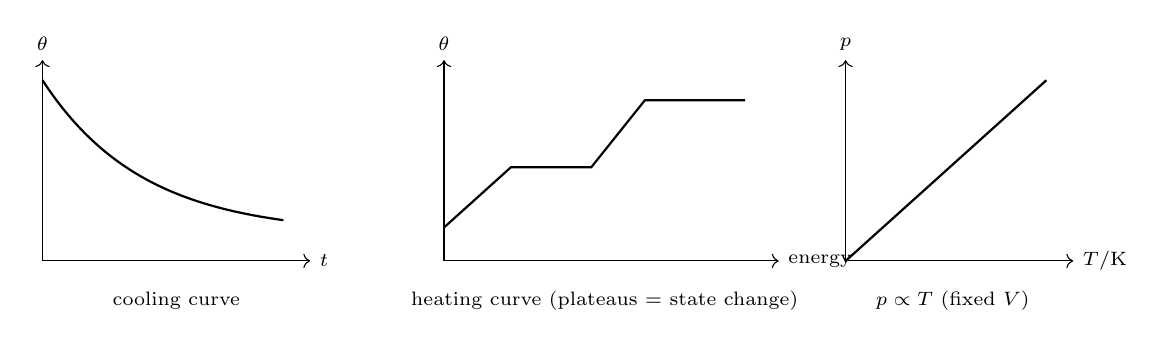
\begin{tikzpicture}[scale=0.85]
% cooling curve
\begin{scope}
\draw[->] (0,0)--(4,0) node[right]{\scriptsize $t$};
\draw[->] (0,0)--(0,3) node[above]{\scriptsize $\theta$};
\draw[thick,domain=0:3.6,samples=40,smooth] plot (\x,{0.4+2.3*exp(-\x/1.5)});
\node at (2,-0.6){\scriptsize cooling curve};
\end{scope}
% heating curve with plateaus
\begin{scope}[xshift=6cm]
\draw[->] (0,0)--(5,0) node[right]{\scriptsize energy};
\draw[->] (0,0)--(0,3) node[above]{\scriptsize $\theta$};
\draw[thick] (0,0.5)--(1,1.4)--(2.2,1.4)--(3,2.4)--(4.5,2.4);
\node at (2.4,-0.6){\scriptsize heating curve (plateaus $=$ state change)};
\end{scope}
% p vs T
\begin{scope}[xshift=12cm]
\draw[->] (0,0)--(3.4,0) node[right]{\scriptsize $T$/K};
\draw[->] (0,0)--(0,3) node[above]{\scriptsize $p$};
\draw[thick] (0,0)--(3,2.7);
\node at (1.6,-0.6){\scriptsize $p\propto T$ (fixed $V$)};
\end{scope}
\end{tikzpicture}
\end{center}

\vspace{0.6cm}
\begin{plainbox}
\textbf{Closing reminder.} The examiner is testing whether you can say the \emph{right
keywords in the right order}. Rehearse the conduction, convection and radiation chains, the
emit/absorb/reflect distinctions, and the insulation logic until they are automatic ---
then the calculations ($\dE=mc\,\dtheta$, $\dE=L\,\Delta m$) are quick marks with a clean
layout.
\end{plainbox}

\end{document}
